\documentclass[../../main.tex]{subfiles}
\begin{document}

\begin{flushright}
  \footnotesize\textit{【自動文字起こし・要確認】}
\end{flushright}

[解]
\paragraph{(1)}

$\vec{c} =
\begin{pmatrix} p \\ q \\ r
\end{pmatrix}$ とおく．($p^2+q^2+r^2=1$, $p,q,r \in \mathbb{R}$)．$|\vec{a}|=|\vec{b}|=|\vec{c}|=1$ から，$\alpha, \beta$ は各々 $\vec{a}$ と $\vec{c}$, $\vec{b}$ と $\vec{c}$ のなす角にひとしい．
\begin{figure}[htb]
  \centering
  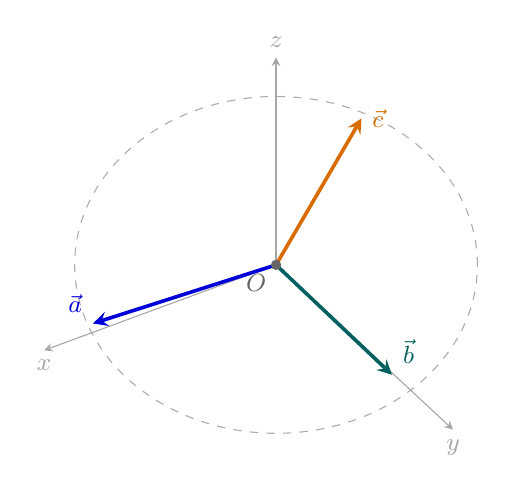
\begin{tikzpicture}[scale=1.55, >=stealth, every node/.style={font=\small}]
    \coordinate (O) at (0,0);
    \coordinate (A) at (-1.5,-0.48);
    \coordinate (B) at (0.95,-0.9);
    \coordinate (C) at (0.7,1.2);
    \draw[dashed, gray!65] (O) ellipse[x radius=1.65, y radius=1.38];
    \draw[->, gray!70] (O) -- (-1.9,-0.7) node[below] {$x$};
    \draw[->, gray!70] (O) -- (1.45,-1.35) node[below] {$y$};
    \draw[->, gray!70] (O) -- (0,1.7) node[above] {$z$};
    \draw[->, line width=1.3pt, blue!85!black] (O) -- (A) node[above left] {$\vec a$};
    \draw[->, line width=1.3pt, teal!75!black] (O) -- (B) node[above right] {$\vec b$};
    \draw[->, line width=1.3pt, orange!85!black] (O) -- (C) node[right] {$\vec c$};
    \fill[gray!80!black] (O) circle (1.2pt) node[below left] {$O$};
  \end{tikzpicture}
  \caption{共通の始点をもつ3本の単位ベクトルと角$\alpha,\beta$}
\end{figure}
\begin{align}
  \cos\alpha &=
  \begin{pmatrix} 1 \\ 0 \\ 0
  \end{pmatrix} \cdot
  \begin{pmatrix} p \\ q \\ r
  \end{pmatrix} = p \\
  \cos\beta &=
  \begin{pmatrix} 1/2 \\ \sqrt{3}/2 \\ 0
  \end{pmatrix} \cdot
  \begin{pmatrix} p \\ q \\ r
  \end{pmatrix} = \dfrac{1}{2}p + \dfrac{\sqrt{3}}{2}q
\end{align}
だから，
\begin{align}
  (与式左辺) &= p^2 - \dfrac{1}{2}p^2 - \dfrac{\sqrt{3}}{2}pq + \dfrac{1}{4}(p+\sqrt{3}q)^2 \\
  &= \dfrac{1}{2}p^2 - \dfrac{\sqrt{3}}{2}pq + \dfrac{1}{4}p^2 + \dfrac{\sqrt{3}}{2}pq + \dfrac{3}{4}q^2 \\
  &= \dfrac{3}{4}(p^2+q^2) \le \dfrac{3}{4}(p^2+q^2+r^2) = \dfrac{3}{4} \ (\because r \in \mathbb{R}, =)
\end{align}

[(1)別] (すがキエルのパラメーター表示でもOK)

\paragraph{(2)}

$t = \cos\alpha, s = \cos\beta$ とおく．(1) から
\begin{align}
  &s^2 - ts + t^2 - \dfrac{3}{4} \le 0 \\
  &\dfrac{1}{2}(t - \sqrt{3}| \sin\alpha |) \le s \le \dfrac{1}{2}(t + \sqrt{3}| \sin\alpha |)
\end{align}
$0 \le \alpha \le \pi$ から $\sin\alpha \ge 0$ だから
\begin{align}
  &\dfrac{1}{2}(\cos\alpha - \sqrt{3}\sin\alpha) \le \cos\beta \le (\cos\alpha + \sqrt{3}\sin\alpha)/2 \\
  &\cos\left(\alpha + \dfrac{\pi}{3}\right) \le \cos\beta \le \cos\left(\alpha - \dfrac{\pi}{3}\right)
\end{align}
$0 \le \beta \le \pi$ では $\cos\beta$ は単調減少だから

\begin{figure}[htb]
  \centering
  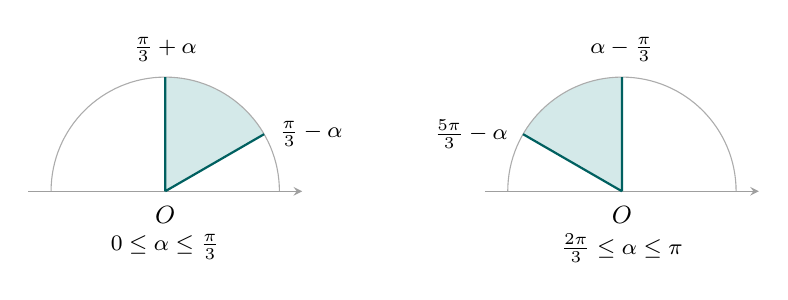
\begin{tikzpicture}[scale=1.45, >=stealth, every node/.style={font=\small}]
    \begin{scope}
      \fill[teal!17] (0,0) -- (30:1) arc[start angle=30,end angle=90,radius=1] -- cycle;
      \draw[gray!65] (1,0) arc[start angle=0,end angle=180,radius=1];
      \draw[->, gray!75] (-1.2,0) -- (1.2,0);
      \draw[teal!75!black, thick] (0,0) -- (30:1) (0,0) -- (90:1);
      \node[below=2pt] at (0,0) {$O$};
      \node[right=2pt, font=\footnotesize] at (30:1) {$\frac{\pi}{3}-\alpha$};
      \node[above=2pt, font=\footnotesize] at (90:1) {$\frac{\pi}{3}+\alpha$};
      \node[below=12pt, font=\footnotesize] at (0,0) {$0\leq\alpha\leq\frac{\pi}{3}$};
    \end{scope}
    \begin{scope}[shift={(4,0)}]
      \fill[teal!17] (0,0) -- (90:1) arc[start angle=90,end angle=150,radius=1] -- cycle;
      \draw[gray!65] (1,0) arc[start angle=0,end angle=180,radius=1];
      \draw[->, gray!75] (-1.2,0) -- (1.2,0);
      \draw[teal!75!black, thick] (0,0) -- (90:1) (0,0) -- (150:1);
      \node[below=2pt] at (0,0) {$O$};
      \node[above=2pt, font=\footnotesize] at (90:1) {$\alpha-\frac{\pi}{3}$};
      \node[left=2pt, font=\footnotesize] at (150:1) {$\frac{5\pi}{3}-\alpha$};
      \node[below=12pt, font=\footnotesize] at (0,0) {$\frac{2\pi}{3}\leq\alpha\leq\pi$};
    \end{scope}
  \end{tikzpicture}
  \caption{$\alpha$の範囲によって変わる$\beta$の許容角（代表例）}
\end{figure}

$1^\circ$ $0 \le \alpha \le \dfrac{\pi}{3}$ の時
\[ \dfrac{\pi}{3} - \alpha \le \beta \le \alpha + \dfrac{\pi}{3} \]

$2^\circ$ $\dfrac{\pi}{3} \le \alpha \le \dfrac{2}{3}\pi$ の時
\[ \alpha + \dfrac{\pi}{3} \ge \beta \ge \alpha - \dfrac{\pi}{3} \]

$3^\circ$ $\dfrac{2}{3}\pi \le \alpha \le \pi$ の時
\[ \alpha - \dfrac{\pi}{3} \le \beta \le -\alpha + \dfrac{5}{3}\pi \]

\begin{figure}[htb]
  \centering
  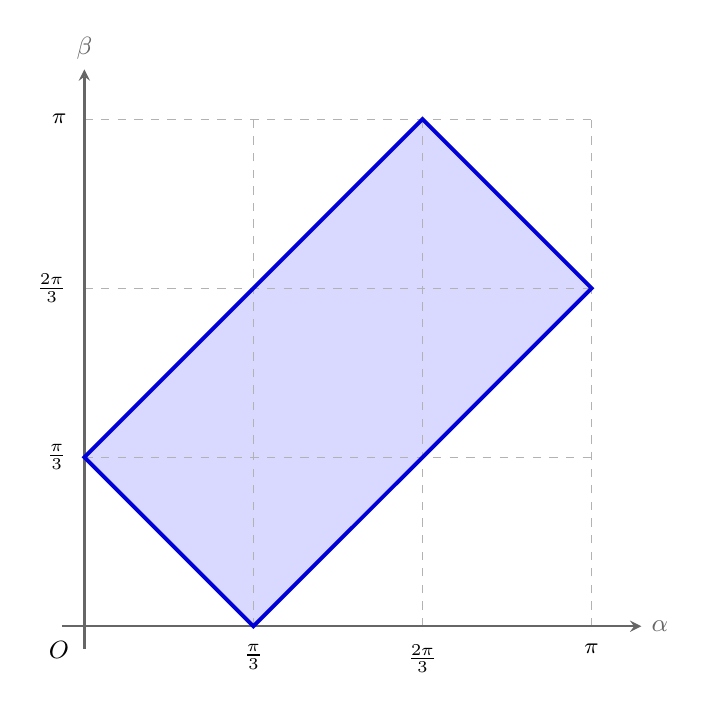
\begin{tikzpicture}[x=2.05cm, y=2.05cm, >=stealth, every node/.style={font=\small}]
    \fill[blue!15] (0,1.047) -- (1.047,0) -- (3.142,2.094) -- (2.094,3.142) -- cycle;
    \foreach \v in {1.047,2.094,3.142} {
      \draw[dashed, gray!60] (\v,0) -- (\v,3.142);
      \draw[dashed, gray!60] (0,\v) -- (3.142,\v);
    }
    \draw[->, thick, gray!80!black] (-0.14,0) -- (3.45,0) node[right] {$\alpha$};
    \draw[->, thick, gray!80!black] (0,-0.14) -- (0,3.45) node[above] {$\beta$};
    \draw[line width=1.4pt, blue!85!black]
    (0,1.047) -- (1.047,0) -- (3.142,2.094) -- (2.094,3.142) -- cycle;
    \node[below=3pt, font=\footnotesize] at (1.047,0) {$\frac{\pi}{3}$};
    \node[below=3pt, font=\footnotesize] at (2.094,0) {$\frac{2\pi}{3}$};
    \node[below=3pt, font=\footnotesize] at (3.142,0) {$\pi$};
    \node[left=3pt, font=\footnotesize] at (0,1.047) {$\frac{\pi}{3}$};
    \node[left=3pt, font=\footnotesize] at (0,2.094) {$\frac{2\pi}{3}$};
    \node[left=3pt, font=\footnotesize] at (0,3.142) {$\pi$};
    \node[below left=2pt] at (0,0) {$O$};
  \end{tikzpicture}
  \caption{$0\leq\alpha,\beta\leq\pi$で成り立つ領域（境界を含む）}
\end{figure}
(図示して下図斜線部(境界含む))

\end{document}
